\documentclass[12pt,a4paper]{article}
\usepackage[utf8]{vietnam}
\usepackage{amsmath,amssymb,amsfonts,amsthm}
\usepackage{graphicx}
\usepackage{tabularray}
\usepackage{tabularx}
\usepackage{tikz}
\usetikzlibrary{calc}
\usepackage[left=2.5cm,right=2cm,top=2.5cm,bottom=2.5cm]{geometry}
\usepackage{fancyhdr}
\setlength{\headheight}{15.2807pt}
\usepackage{xcolor}
\usepackage{array}
\usepackage{titlesec}
\usepackage{hyperref}
\usepackage{float}
\usepackage{caption}
\usepackage{subcaption}
\usepackage{booktabs}
\usepackage{enumitem}
\usepackage{indentfirst}
\captionsetup[figure]{justification=centering}
\usepackage{minted}
\setminted{style=friendly}

% ===== Code block style (tcolorbox + minted) =====
\usepackage{tcolorbox}
\tcbuselibrary{minted,breakable,xparse,skins}
\definecolor{bg}{gray}{0.95}
\DeclareTCBListing{mintedbox}{O{}m!O{}}{%
  breakable=true,
  listing engine=minted,
  listing only,
  minted language=#2,
  minted style=friendly,
  minted options={%
    linenos,
    gobble=0,
    breaklines=true,
    breakafter=,,
    fontsize=\small,
    numbersep=8pt,
    #1},
  boxsep=0pt,
  left skip=0pt,
  right skip=0pt,
  left=25pt,
  right=0pt,
  top=3pt,
  bottom=3pt,
  arc=5pt,
  leftrule=0pt,
  rightrule=0pt,
  bottomrule=2pt,
  toprule=2pt,
  colback=bg,
  colframe=orange!70,
  enhanced,
  overlay={%
    \begin{tcbclipinterior}
    \fill[orange!20!white] (frame.south west) rectangle ([xshift=20pt]frame.north west);
    \end{tcbclipinterior}},
  #3}

% ===== Hyperlink =====
\hypersetup{
    colorlinks=true,
    linkcolor=blue!70!black,
    filecolor=magenta,
    urlcolor=cyan,
    citecolor=red!70!black
}

% ===== Header / Footer =====
\pagestyle{fancy}
\fancyhf{}
\lhead{\textbf{Báo cáo BTVN -- Vật lý tính toán}}
\rhead{\textit{Phương trình sóng 1D -- FTCS}}
\cfoot{\thepage}
\renewcommand{\headrulewidth}{0.4pt}
\renewcommand{\footrulewidth}{0.4pt}

% ===== Section formatting =====
\titleformat{\section}{\Large\bfseries\color{blue!80!black}}{\thesection.}{0.5em}{}
\titleformat{\subsection}{\large\bfseries\color{blue!70!black}}{\thesubsection.}{0.5em}{}
\titleformat{\subsubsection}{\normalsize\bfseries\color{blue!60!black}}{\thesubsubsection.}{0.5em}{}

\begin{document}

% ================= TRANG BÌA =================
\begin{titlepage}
    \centering
    \vspace*{2cm}
    \rule{\textwidth}{1pt} \\[0.5cm]
    {\huge \textbf{BÁO CÁO BÀI TẬP VỀ NHÀ}} \\[0.4cm]
    {\large \textbf{GIẢI PHƯƠNG TRÌNH SÓNG 1D BẰNG}} \\[0.2cm]
    {\large \textbf{PHƯƠNG PHÁP SAI PHÂN HỮU HẠN HIỆN (FTCS)}} \\[0.2cm]
    \rule{\textwidth}{1pt}

    \vspace{2cm}

    {\large
    \begin{tabular}{rl}
        \textbf{Họ và tên:}  & Nguyễn Trần Gia Bảo \\[4pt]
        \textbf{MSSV:}       & 23137003 \\[4pt]
        \textbf{Môn học:}    & Vật lý tính toán (PHY10532) \\[4pt]
        \textbf{Giảng viên:} & TS.\@ Vũ Quang Tuyên \\
    \end{tabular}
    }

    \vfill
    {\large \today}
\end{titlepage}

% ================= MỤC LỤC =================
\newpage
\tableofcontents
\newpage

% =============================================================
\section{Cơ sở lý thuyết}

\subsection{Phương trình sóng 1D}

Phương trình sóng truyền trên một sợi dây hai đầu cố định không có ma sát:
\begin{equation}
\frac{\partial^2 u(x,t)}{\partial t^2} = c^2\,\frac{\partial^2 u(x,t)}{\partial x^2},\qquad c=\sqrt{T/\rho},
\end{equation}
với $T=40\text{ N}$, $\rho=0.01\text{ kg/m}$, $L=1\text{ m}$. Khi tính đến lực ma sát tỉ lệ và ngược chiều vận tốc, phương trình trở thành:
\begin{equation}
\frac{\partial^2 u}{\partial t^2} = c^2\,\frac{\partial^2 u}{\partial x^2} - \frac{2\kappa}{\rho}\,\frac{\partial u}{\partial t}.
\end{equation}

\subsection{Sai phân hữu hạn hiện (FTCS)}

Đặt $\beta = ck/h$ với $k=\Delta t$, $h=\Delta x$. Sai phân trung tâm cho cả hai đạo hàm bậc hai cho công thức:
\begin{equation}
u_{i+1,j} = 2(1-\beta^2)\,u_{i,j} + \beta^2(u_{i,j+1}+u_{i,j-1}) - u_{i-1,j}.
\end{equation}
Khi có ma sát, với $\gamma = 2\kappa k/\rho$:
\begin{equation}
u_{i+1,j} = (2-\gamma)\,u_{i,j} + (\gamma-1)\,u_{i-1,j} + \beta^2(u_{i,j+1}-2u_{i,j}+u_{i,j-1}).
\end{equation}
\textbf{Điều kiện ổn định Courant:} $\beta = ck/h \le 1$.

\subsection{Điều kiện đầu, điều kiện biên}

\begin{itemize}[leftmargin=*]
    \item Hình dạng đầu: $u(x,0)=f(x)$.
    \item Vận tốc ban đầu bằng 0: $\partial u/\partial t\big|_{t=0}=g(x)=0$ $\Rightarrow$ $u_{1,j}\approx u_{0,j} + k\,g(x_j)$ (gần đúng bậc 1).
    \item Biên cố định: $u(0,t)=u(L,t)=0$.
\end{itemize}

% =============================================================
\section{Thực hành 1 -- Phương trình sóng không và có ma sát}

\subsection{Hàm khởi tạo và sai phân hiện}

\begin{mintedbox}{python}
def khoitao_u(dt, dx, tmax, L, f_x, g_x):
    n = int(tmax/dt) + 1
    m = int(L/dx) + 1
    u = np.zeros((n, m))
    x = np.linspace(0, L, m)
    t = np.linspace(0, tmax, n)
    for j in range(m):
        u[0, j] = f_x(x[j], L)
        u[1, j] = u[0, j] + dt * g_x(x[j], L)
    u[:, 0]  = 0.0
    u[:, -1] = 0.0
    return u, x, t

def ham_forward_khong_friction(c, k, h, tmax, L, f_x, g_x, filename):
    u, x, t = khoitao_u(k, h, tmax, L, f_x, g_x)
    n, m = u.shape
    beta, ondinh = tinh_beta(c, k, h)
    if ondinh:
        for i in range(1, n-1):
            for j in range(1, m-1):
                u[i+1, j] = 2*(1-beta**2)*u[i,j] + beta**2*(u[i,j+1]+u[i,j-1]) - u[i-1,j]
        ghifile(u, x, t, beta, filename)
\end{mintedbox}

\subsection{Bài toán gốc -- gảy dây tại $x=0.8L$}

Hàm khởi tạo dạng tam giác lệch:
\[
f(x)=\begin{cases}1.25\,x/L & x\le 0.8L,\\ 5-5x/L & x>0.8L,\end{cases}\qquad g(x)=0.
\]

\begin{mintedbox}{python}
def f_x_bai1(x, l):
    if x <= 0.8*l:
        return 1.25*x/l
    else:
        return 5 - 5*x/l
\end{mintedbox}

Vận tốc $c=\sqrt{40/0.01}=63.25\text{ m/s}$. Khảo sát với hai cấu hình:
\begin{itemize}[leftmargin=*]
    \item $\Delta x=0.01\text{ m}$, $\Delta t=10^{-4}\text{ s}$ $\Rightarrow$ $\beta\approx 0.63$ (ổn định).
    \item $\Delta x=0.007\text{ m}$, $\Delta t=10^{-4}\text{ s}$ $\Rightarrow$ $\beta\approx 0.90$ (ổn định).
\end{itemize}

\begin{figure}[H]
    \centering
    
\includegraphics[width=0.95\textwidth]{wave_3d.pdf}
    \caption{Mặt $u(x,t)$ với $\beta=0.63$ (trái) và $\beta=0.90$ (phải). Cả hai đều ổn định; sóng phản xạ qua lại đối xứng, không suy giảm biên độ.}
    \label{fig:wave3d}
\end{figure}

\textbf{Nhận xét:} Khi $\beta\le 1$ phương pháp ổn định. Thử với $\beta>1$ (chia mịn $\Delta t$ hoặc thô $\Delta x$) thì nghiệm số phân kỳ ngay sau vài bước thời gian -- đúng dự đoán Courant.

\subsection{Điều kiện đầu dạng mode đơn $\sin(\pi x/L)$}

\begin{mintedbox}{python}
def f_x_bai1_ham_sin(x, l):
    return np.sin(x * np.pi / l)
\end{mintedbox}

\begin{figure}[H]
    \centering
    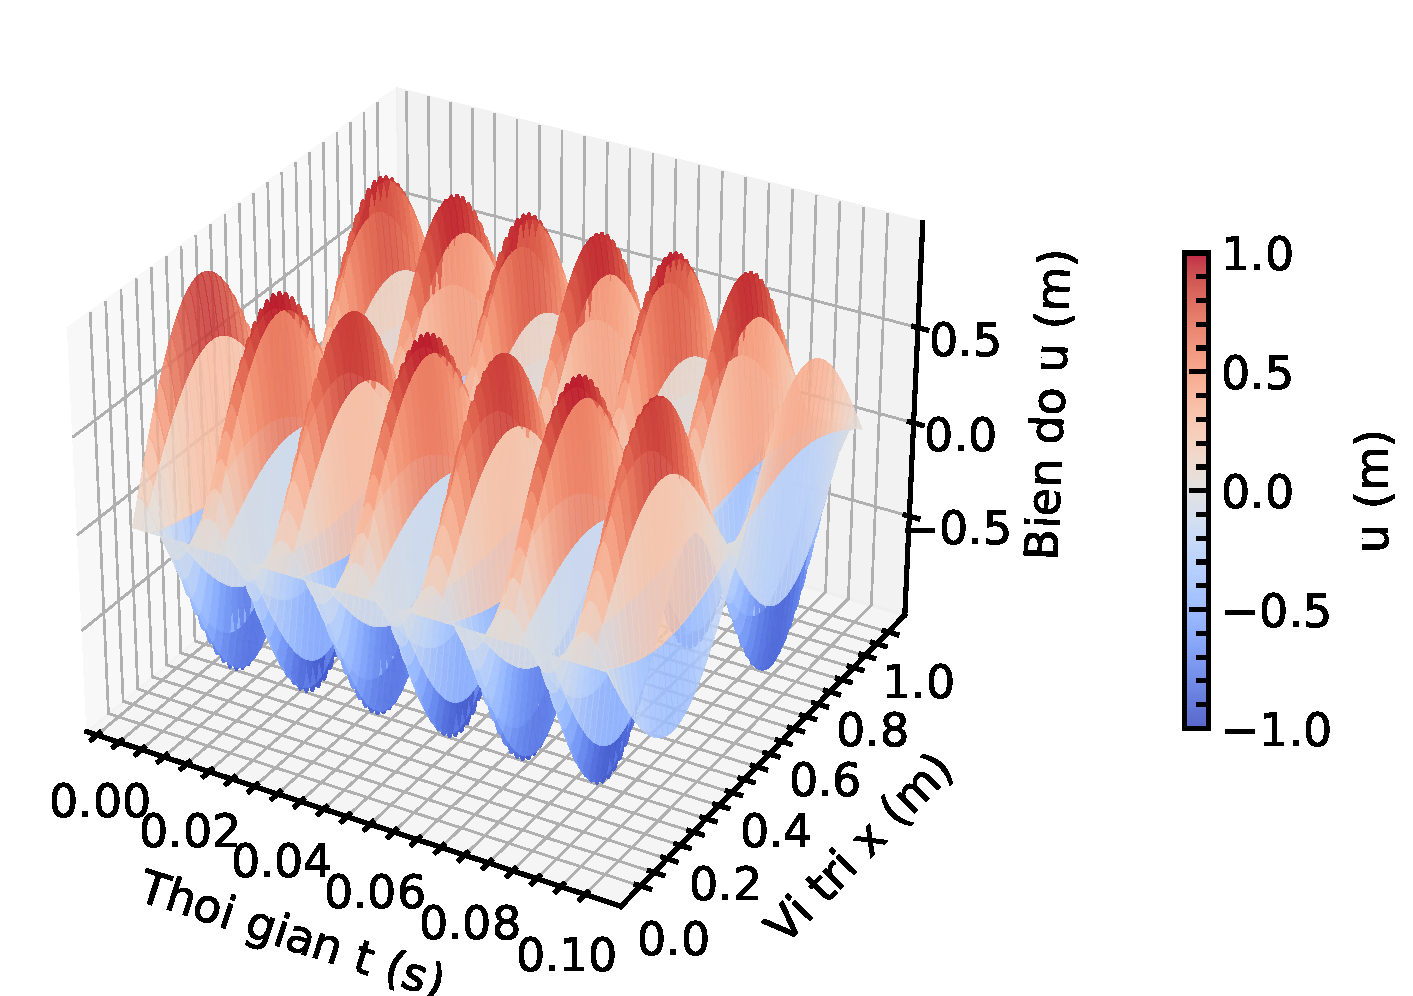
\includegraphics[width=0.62\textwidth]{wave_3d_sin.pdf}
    \caption{Sóng dừng (mode cơ bản) sinh ra khi điều kiện đầu là một mode chuẩn của dây.}
    \label{fig:sin1}
\end{figure}

\textbf{Nhận xét:} Vì $\sin(\pi x/L)$ đã là một nghiệm riêng của bài toán nên kết quả là sóng dừng thuần túy, các điểm nút cố định tại $x=0,L$.

\subsection{Mở rộng -- thêm ma sát}

\begin{mintedbox}{python}
def ham_forward_friction(c, k, h, tmax, L, f_x, g_x, kappa, rho, filename):
    u, x, t = khoitao_u(k, h, tmax, L, f_x, g_x)
    n, m = u.shape
    beta, ondinh = tinh_beta(c, k, h)
    gamma = 2 * kappa * k / rho
    if ondinh:
        for i in range(1, n-1):
            for j in range(1, m-1):
                lap = u[i, j+1] - 2*u[i, j] + u[i, j-1]
                u[i+1, j] = (2-gamma)*u[i,j] + (gamma-1)*u[i-1,j] + beta**2*lap
        ghifile(u, x, t, beta, filename)
    return u, x, t
\end{mintedbox}

Khảo sát $\kappa\in\{0.01,\,1,\,2,\,5,\,10\}$ với điều kiện đầu gốc (gảy tại $0.8L$):

\begin{figure}[H]
    \centering
    \includegraphics[width=0.95\textwidth]{wave_all_kappa.pdf}
    \caption{Ảnh hưởng của hệ số ma sát $\kappa$ lên dao động dây. Biên độ tắt dần theo thời gian; $\kappa$ càng lớn thì sóng tắt càng nhanh.}
    \label{fig:kappa}
\end{figure}

\textbf{Nhận xét:} Với $\kappa$ nhỏ ($0.01$) dây gần như dao động tự do; tăng $\kappa$ làm biên độ giảm theo dạng tắt dần mũ, đúng bản chất số hạng $-(2\kappa/\rho)\,\partial u/\partial t$.

% =============================================================
\section{Thực hành 2 -- Các yêu cầu 3--7 (sách Landau, 2015)}

\subsection{Yêu cầu 3 -- So sánh nghiệm giải tích và nghiệm số}

Khai triển Fourier với điều kiện đầu gảy lệch:
\begin{equation}
u(x,t)=\sum_{n=1}^{\infty} B_n \sin\!\left(\frac{n\pi x}{L}\right)\cos\!\left(\frac{cn\pi t}{L}\right),\quad B_n=\frac{12.5\,\sin(0.8n\pi)}{n^2\pi^2}.
\end{equation}

\begin{mintedbox}{python}
def nghiem_giai_tich(x, t, L):
    u = 0
    for n in range(1, 200):
        B_n = 12.5*np.sin(np.pi*n*0.8)/(n*np.pi)**2
        u += B_n * np.sin(n*np.pi*x/L) * np.cos(c*n*np.pi*t/L)
    return u
\end{mintedbox}

\begin{figure}[H]
    \centering
    
\includegraphics[width=0.7\textwidth]{hinh_dang_soi_day.pdf}
    \caption{Hình dạng sợi dây ở các thời điểm khác nhau: nét liền -- giải tích (tổng 200 mode), nét đứt -- giải số ($\beta=0.90$).}
    \label{fig:compare}
\end{figure}

\textbf{Nhận xét:} Hai nghiệm trùng khớp tốt; sai khác chủ yếu xuất hiện ở các đỉnh nhọn do hiệu ứng Gibbs trong chuỗi Fourier hữu hạn.

\subsection{Yêu cầu 4 -- Ước lượng vận tốc truyền sóng $c$}

Vẽ vị trí biên độ đỉnh sóng theo thời gian, sau đó hồi quy tuyến tính trên đoạn $t\in[0.1,\,7.8]\text{ ms}$:

\begin{figure}[H]
    \centering
    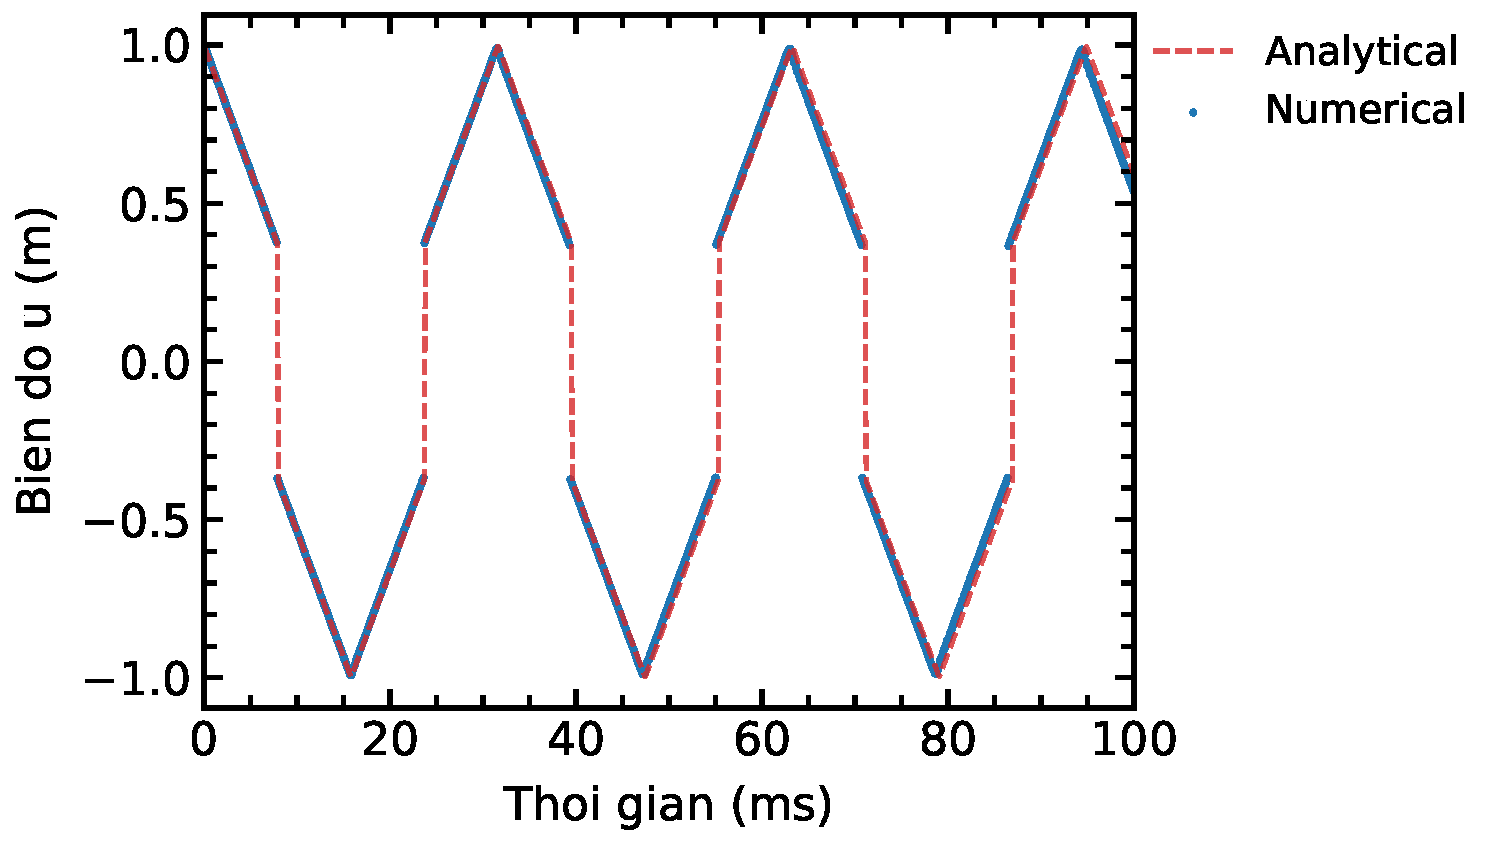
\includegraphics[width=0.6\textwidth]{dinh_song_full_sosanh.pdf}
    \caption{Biên độ đỉnh sóng theo thời gian -- so sánh nghiệm số và nghiệm giải tích.}
    \label{fig:peak_amplitude}
\end{figure}

\begin{figure}[H]
    \centering
    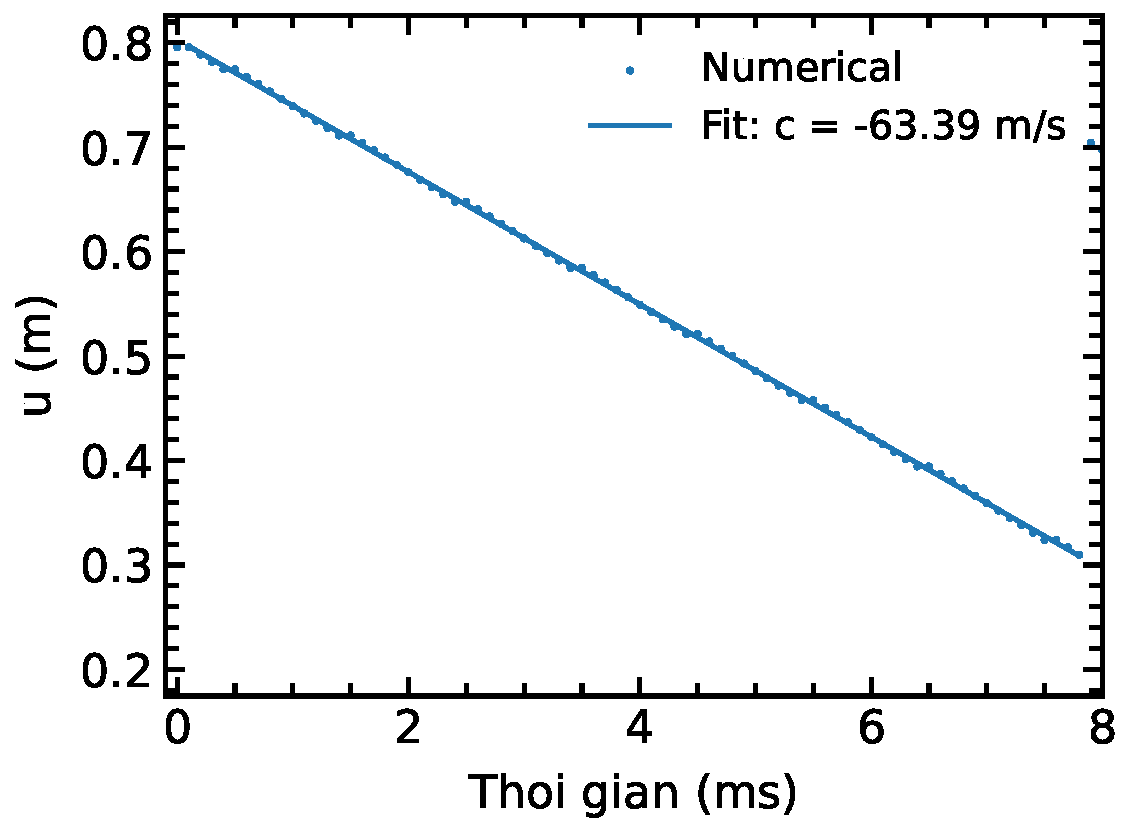
\includegraphics[width=0.6\textwidth]{hoi_quy_van_toc.pdf}
    \caption{Hồi quy tuyến tính vị trí đỉnh sóng theo thời gian để ước lượng vận tốc truyền sóng $c$.}
    \label{fig:velocity_fit}
\end{figure}

\textbf{Kết quả:} $c_{\text{số}} \approx 63.2\text{ m/s}$, gần như trùng với giá trị lý thuyết $c=\sqrt{T/\rho}=63.25\text{ m/s}$.
Sai khác $\sim 0.1\%$.

\subsection{Yêu cầu 5 -- Mode chuẩn cho ra sóng dừng}

Thử với các mode bậc cao $\sin(2\pi x/L)$ và $\sin(3\pi x/L)$:

\begin{figure}[H]
    \centering
    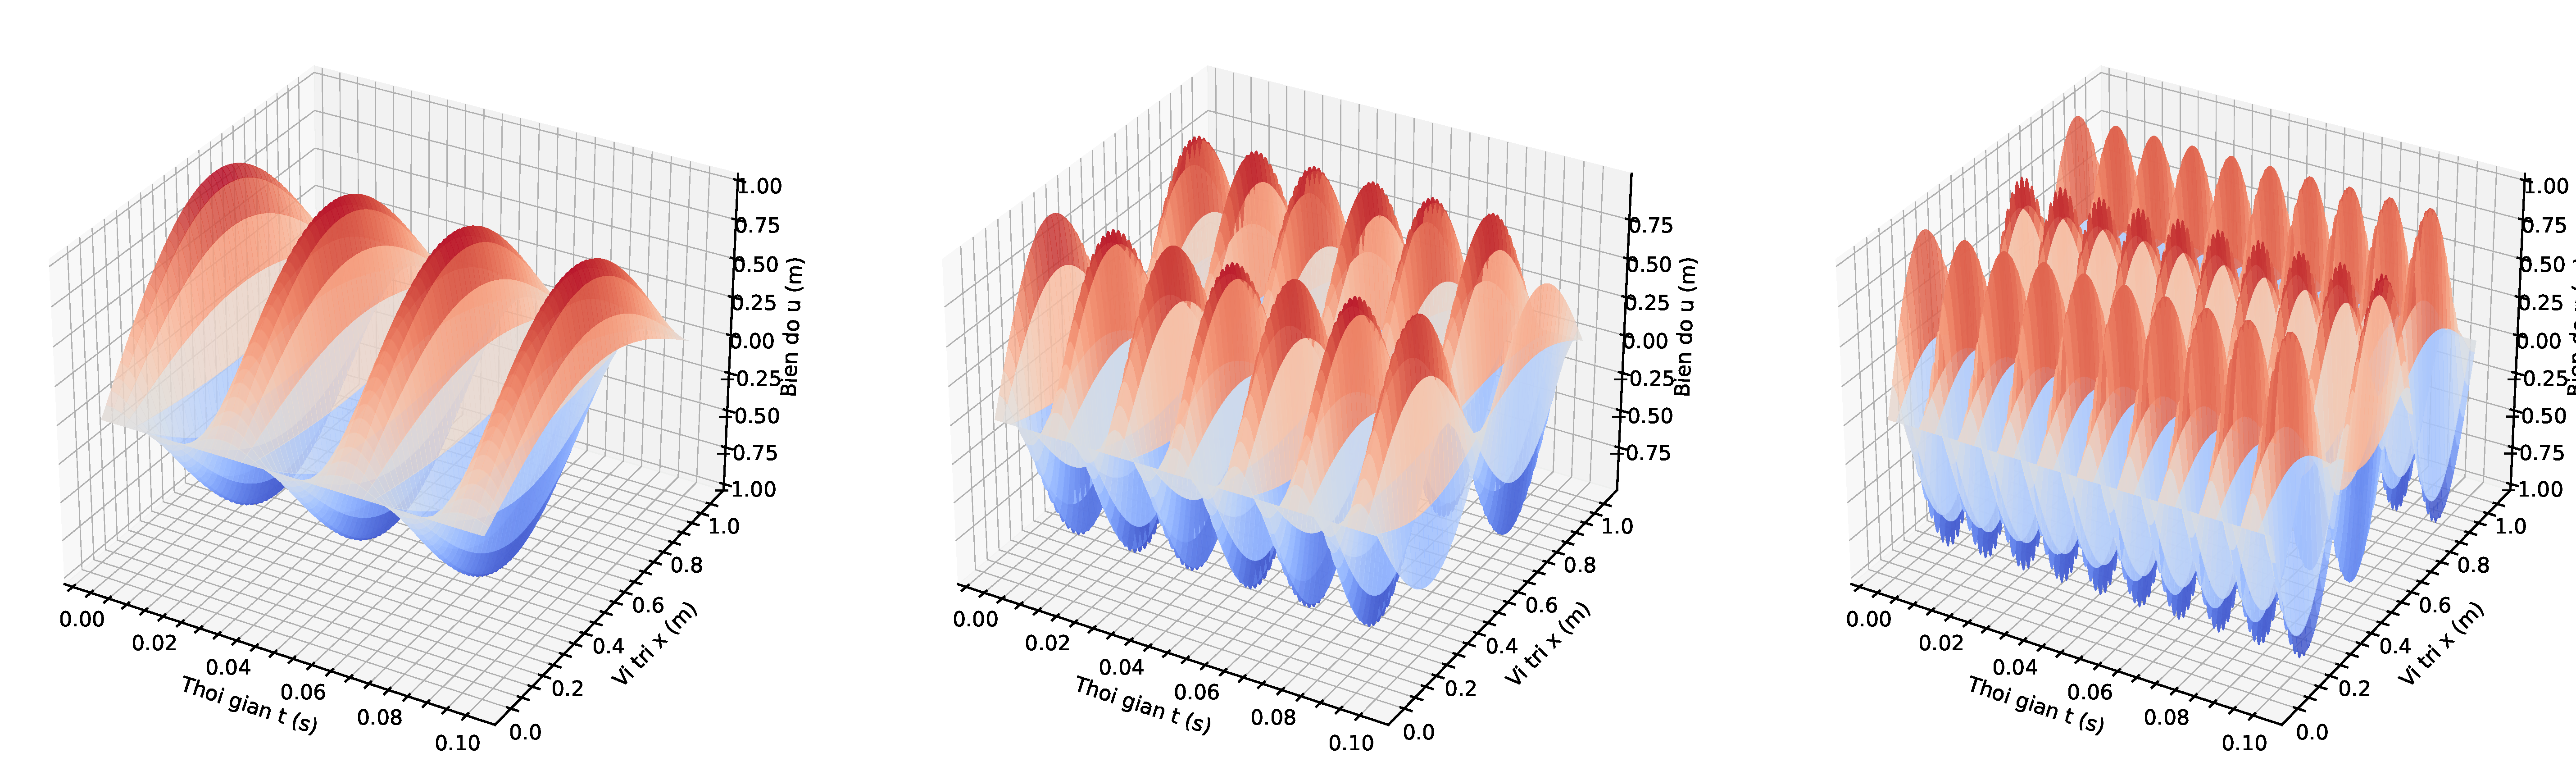
\includegraphics[width=0.95\textwidth]{wave_songdung_bai2.pdf}
    \caption{Sóng dừng với mode $n=1,\,2,\,3$. Mode $n$ có $n+1$ điểm nút (kể cả hai đầu).}
    \label{fig:modes}
\end{figure}

\textbf{Nhận xét:} Khi điều kiện đầu là một mode chuẩn đơn lẻ, kết quả số đúng là sóng dừng với tần số $\omega_n=cn\pi/L$, các nút cố định -- phù hợp lý thuyết.

\subsection{Yêu cầu 6 -- Hiện tượng phách (beating)}

Cho điều kiện ban đầu là tổng hai mode chuẩn: $\sin(\pi x/L)+\sin(2\pi x/L)$ và $\sin(\pi x/L)+\sin(3\pi x/L)$.

\begin{figure}[H]
    \centering
    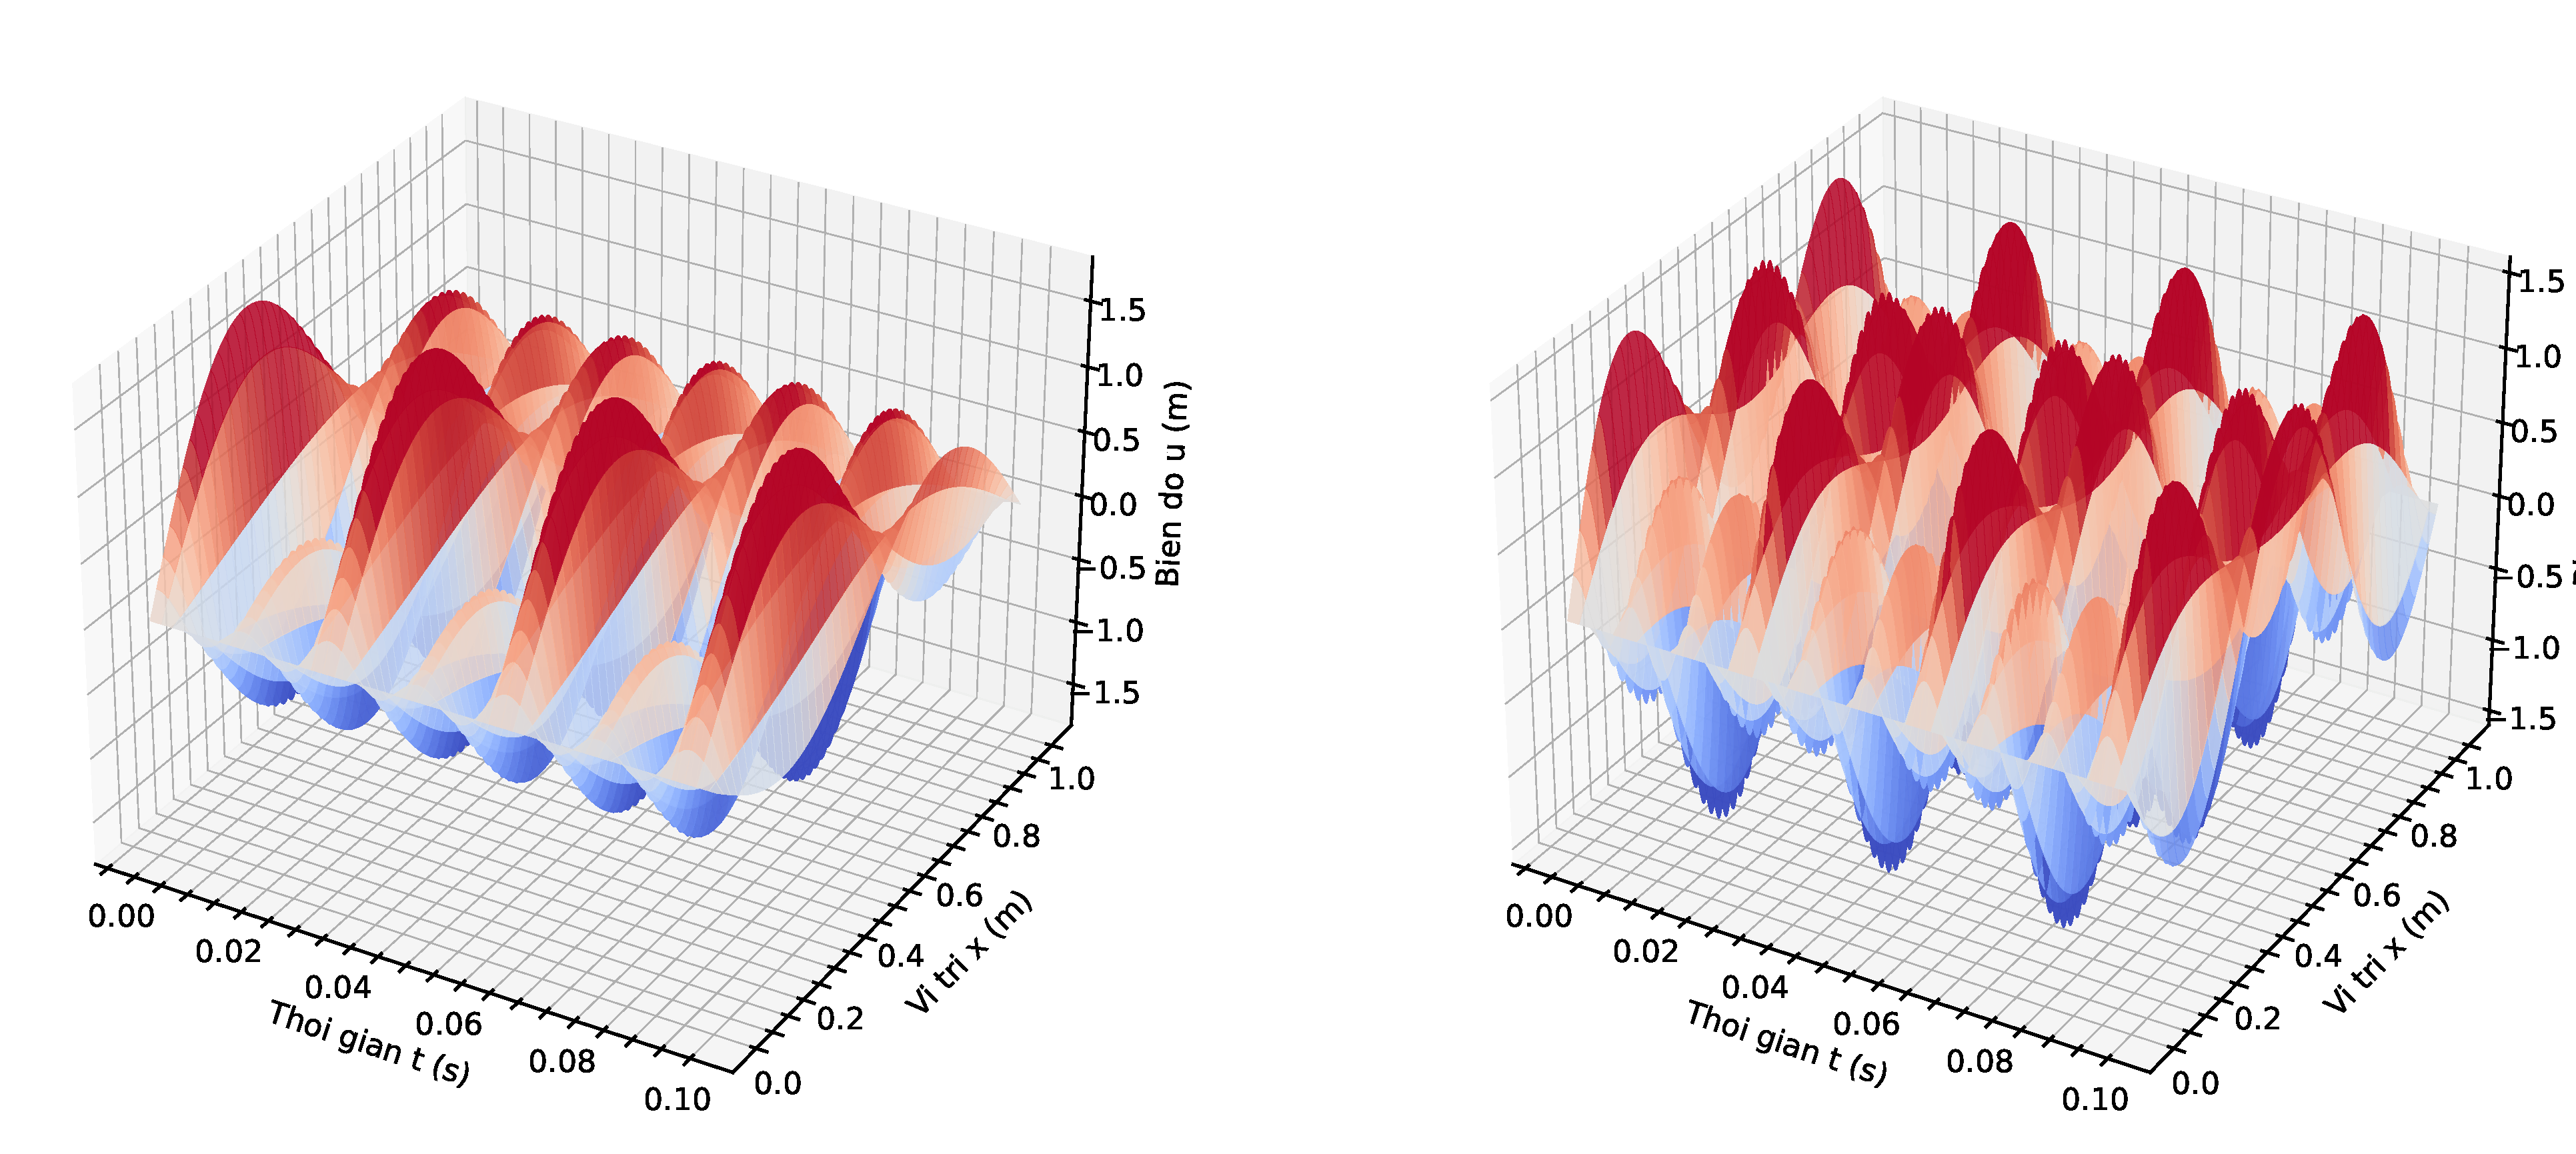
\includegraphics[width=0.95\textwidth]{wave_hientuong_phach_bai2.pdf}
    \caption{Tổ hợp hai mode liền kề tạo nên hiện tượng phách -- biên độ tổng dao động tuần hoàn với tần số phách $\Delta\omega = c(n_2-n_1)\pi/L$.}
    \label{fig:beating}
\end{figure}

\textbf{Nhận xét:} Có hiện tượng phách rõ rệt; chu kỳ phách ngắn hơn khi hai mode cách xa nhau ($n=1,3$) so với trường hợp liền kề ($n=1,2$).

\subsection{Yêu cầu 7 -- Gảy chính giữa dây}

\begin{mintedbox}{python}
def f_x_bai2_songdung(x, l):
    if x <= 0.5*l:
        return 1.25*x/l
    else:
        return 1.25*(l-x)/l
\end{mintedbox}

\begin{figure}[H]
    \centering
    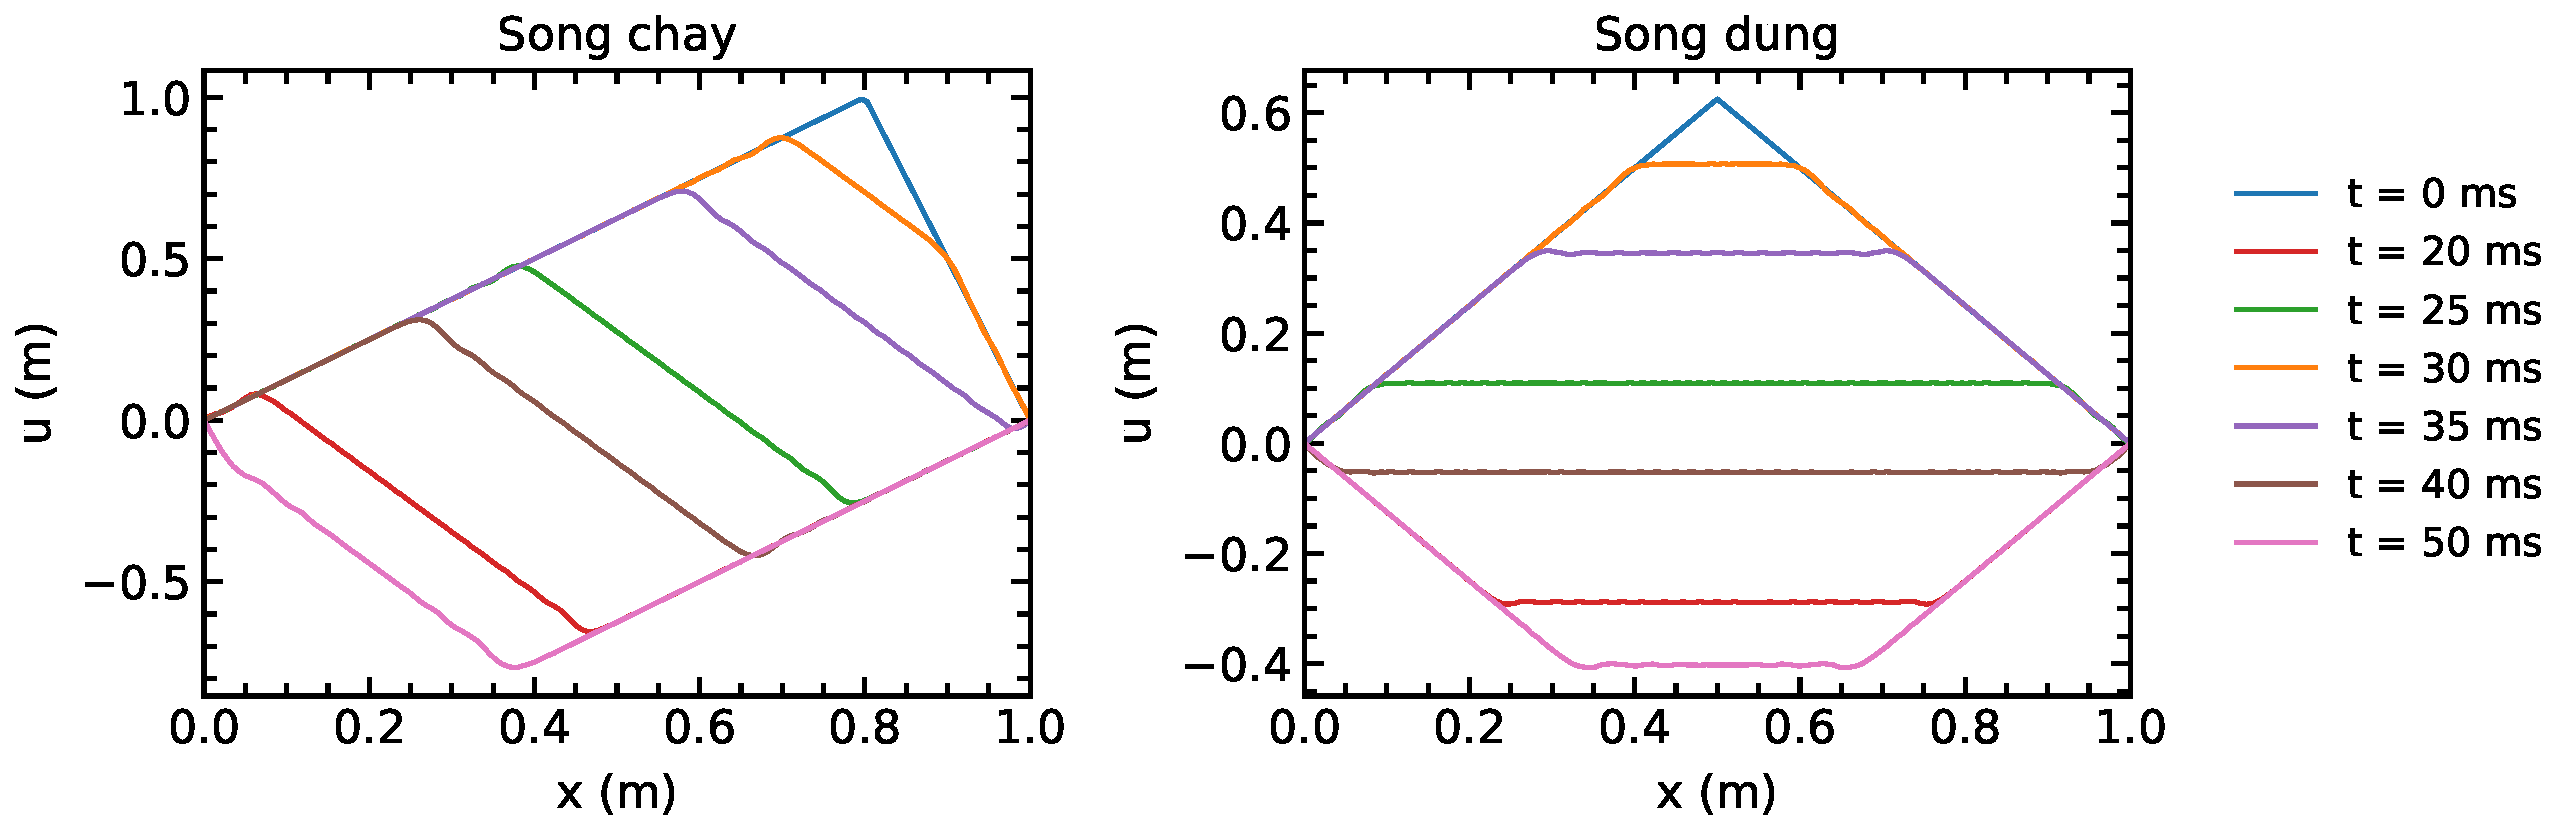
\includegraphics[width=1.0\textwidth]{hinh_dang_soi_day_songdung_songchay.pdf}
    \caption{So sánh: trái -- gảy lệch ($0.8L$) cho sóng chạy; phải -- gảy chính giữa ($0.5L$) cho dạng giống sóng dừng đối xứng.}
    \label{fig:middle}
\end{figure}

\textbf{Nhận xét:} Khi gảy giữa dây, do tính đối xứng của $f(x)$ quanh $x=L/2$, các mode chẵn bị triệt tiêu và chỉ còn các mode lẻ -- kết quả là một sóng đối xứng dao động lên xuống tại chỗ, gần giống sóng dừng (không có đỉnh sóng \emph{chạy} qua lại như trường hợp gảy lệch).

% =============================================================
\section{Thực hành 3 -- Cải tiến điều kiện đầu cho dây có ma sát}

\subsection{Công thức cải tiến}

Khai triển Taylor đến bậc hai và thay $\partial^2 u/\partial t^2|_{t=0} = c^2 f''(x)$:
\begin{equation}
u(x,t_1) = f(x) + k\,g(x) + \frac{c^2 k^2}{2}\,f''(x) + O(k^3).
\end{equation}
Thay $f''(x)$ bằng sai phân trung tâm:
\begin{equation}
\boxed{\;u_{i,1} = (1-\beta^2)\,f(x_i) + \frac{\beta^2}{2}\bigl[f(x_{i+1}) + f(x_{i-1})\bigr] + k\,g(x_i)\;}
\end{equation}

\subsection{Cài đặt}

\begin{mintedbox}{python}
def khoitao_u_caitien_vantoc(dt, dx, tmax, L, f_x, g_x, c, k, h):
    beta, ondinh = tinh_beta(c, k, h)
    if not ondinh:
        return None, None, None
    n = int(tmax/dt) + 1
    m = int(L/dx) + 1
    u = np.zeros((n, m))
    x = np.linspace(0, L, m)
    t = np.linspace(0, tmax, n)
    for j in range(m):
        u[0, j] = f_x(x[j], L)
    for j in range(1, m-1):
        u[1, j] = (1 - beta**2)*u[0, j] \
                + (beta**2/2)*(u[0, j-1] + u[0, j+1]) \
                + dt*g_x(x[j], L)
    u[:, 0]  = 0.0
    u[:, -1] = 0.0
    return u, x, t
\end{mintedbox}

\subsection{So sánh trước và sau cải tiến}

Khảo sát bài toán có ma sát với $\kappa=0.5$, các tham số khác giữ nguyên. So sánh từng điểm giữa lưới $u_{\text{trước}}$ và $u_{\text{sau}}$:

\begin{table}[H]
\centering
\caption{Sai khác giữa nghiệm số trước và sau khi cải tiến điều kiện đầu (${\kappa=0.5}$).}
\begin{tabular}{lc}
\toprule
\textbf{Đại lượng} & \textbf{Giá trị} \\
\midrule
Sai số lớn nhất $\max|\Delta u|$ & $1.1647\times 10^{-2}$ \\
Sai số trung bình $\overline{|\Delta u|}$ & $6.9197\times 10^{-4}$ \\
\bottomrule
\end{tabular}
\end{table}

\textbf{Nhận xét:}
\begin{itemize}[leftmargin=*]
    \item Sai khác trung bình rất nhỏ ($\sim 7\times 10^{-4}$), chứng tỏ ở phần lớn lưới hai phương pháp gần như trùng nhau.
    \item Sai khác lớn nhất $\sim 1.2\times 10^{-2}$ xuất hiện ở vùng đỉnh tam giác (nơi $f''$ kỳ dị) và ở những khoảng thời gian đầu tiên -- đúng vị trí mà bậc gần đúng của $u_{i,1}$ đóng góp mạnh vô biên độ.
    \item Công thức cải tiến chính xác đến $O(k^3)$ trong khi công thức gốc chỉ $O(k^2)$, nên cải tiến giúp giảm sai số ban đầu và cải thiện độ chính xác của nghiệm.
\end{itemize}

% =============================================================
\section{Kết luận}

\begin{itemize}[leftmargin=*]
    \item Phương pháp FTCS giải tốt phương trình sóng 1D khi tuân thủ điều kiện ổn định Courant $\beta=ck/h\le 1$.
    \item Nghiệm số trùng tốt với nghiệm giải tích Fourier (200 mode); vận tốc đỉnh sóng ước lượng từ hồi quy cho $c\approx 63.2\text{ m/s}$, sai khác $\sim 0.1\%$ so với $\sqrt{T/\rho}$.
    \item Các hiện tượng vật lý đặc trưng đều tái hiện đúng: sóng dừng với mode đơn, phách với tổ hợp mode liền kề, tính đối xứng khi gảy giữa dây, và tắt dần khi có ma sát.
    \item Cải tiến điều kiện đầu $u_{i,1}$ bậc cao giảm rõ rệt sai số gần biên đầu của miền thời gian (sai số lớn nhất giảm còn cỡ $10^{-2}$, trung bình cỡ $10^{-4}$).
\end{itemize}

\end{document}